\documentclass[9pt]{IEEEtran}

% basic
\usepackage[english]{babel}
\usepackage{graphicx,epstopdf,fancyhdr,amsmath,amsthm,amssymb,url,array,textcomp,svg,listings,hyperref,xcolor,colortbl,float,gensymb,longtable,supertabular,multicol,placeins}
\usepackage{hyperref}
 % `sumniki' in names
\usepackage[utf8x]{inputenc}

 % search and copy for `sumniki'
\usepackage[T1]{fontenc}
\usepackage{lmodern}
\input{glyphtounicode}
\pdfgentounicode=1
% \usepackage{subfig}
% tidy figures
\graphicspath{{./figures/}}
\DeclareGraphicsExtensions{.pdf,.png,.jpg,.eps}

% correct bad hyphenation here
\hyphenation{op-tical net-works semi-conduc-tor trig-gs}

% ============================================================================================

\title{\vspace{0ex} %
% TITLE IN HERE:
Navigating the government website network using parallel breadth-first crawler
\\ \normalsize{Web Information Extraction and Retrieval 2018/19, Faculty of Computer and Information Science, University of Ljubljana}}
\author{ %
% AUTHOR IN HERE:
Matej Klemen, Andraž Povše, Jaka Stavanja
\vspace{-4.0ex}
}

% ============================================================================================

\begin{document}

\maketitle

\begin{abstract}
In this work we present our implementation of a crawler that navigates the government websites.
It starts from a few given seed pages and crawls pages that are part of the ``\textit{.gov.si}'' network, meanwhile storing binary data and the text on crawled websites.
Using a starting seed of 2 URLs, our crawler visits \textbf{XXX} links, \textbf{[TODO: other stats]}.
\end{abstract}

\section{Introduction}

A web crawler is a program that visits web pages and downloads them for some purpose.
It begins with some amount of seed URLs, which are put into a frontier.
The crawler then selects a web page from frontier according to some strategy, visits the web page and extracts the web page's content and outgoing links.
The outgoing links are put into the frontier and the content is used for some purpose or stored.
This process is then repeated until a certain stopping criteria is reached (e.g. the frontier being empty) \cite{Manning2008}.
The crawling can also be a continuous process (``without end''), but we do not study these in this project. 

In this project we implement a web crawler that crawls Slovenian government websites. 
We are given a set of 4 government websites and choose additional 5 of them and proclaim them as seed websites, from which we start the crawling.
While crawling these websites, our crawler only follows links to other Slovenian government websites.
The crawler crawls these websites, downloads images and files from them and stores them into a database. 
The crawler visits new links in a breadth-first fashion.
We also implement a method to detect near-duplicate websites based on their content.
For this, we use a locality-sensitive hashing algorithm based on min-hashing \cite{Gionis1999}.

The rest of the report is structured as follows.
In chapter \textbf{TODO} we present \textbf{TODO}.
In chapter \textbf{TODO} we present \textbf{TODO} \ldots
In chapter ~\ref{section:database} we present how the database is built.

\section{Crawler}
In this section we present the architecture of the crawler. 
The full source code is available online \footnote{\url{https://github.com/matejklemen/govrilovic}}.

The crawler consists of multiple components: link, sitemap and robots parser, database manager (and the database itself), content deduplicator and a core unit which uses the other components and adds on top of them to produce a parallel crawler that uses breadth first search to navigate the websites.

It takes 4 parameters in total. These are seed pages, maximum number of workers, maximum crawling depth and a flag, determining whether to get files. 
The first two parameters are self-explanatory.
The maximum crawling depth is optional and specifies at what depth we want our crawler to stop. 
If this parameter is not provided, the crawler will stop when there are no more links being produced.

[\textbf{TODO: describe each component briefly - and possibly mention that it's described further in a separate section (if applicable).}]

We used Selenium to make requests, because it also renders the Javascript code on the website. It does, however, not include HTTP status code, which is why we also had to make another request to get that information.

The crawler uses (parallel) breadth-first traversal to crawl the websites. The master (the initial process) keeps a structure with visited links and links that still need to be visited (frontier).
On each level, the frontier is emptied and the links are divided among workers in the following way.
First, the links are grouped by their base domain.
The base domains are split among workers as evenly as possible and the workers then crawl links that were found in previous level for the particular base link.
This means that a certain worker is responsible for crawling links of 1 or more domains.
Each worker keeps a local copy of its visited websites and a local copy of its newly produced links.
Each worker also checks if a newly visited website is present in the global visited structure, but it does not add new links into it as we want to keep the synchronization between workers to a minimum.
We must wait for all the workers to finish so that breadth-first strategy is ensured.
After they are all done, the master collects newly collected links from workers and checks for duplicate links.
It also marks the links from current level as visited.
This process is repeated with the newly collected links, which represent the next level of search process.

While our implementation does not use parallelism as effectively as possible, it does fully respect the crawled sites' rules (for example, the specified crawl delay).
Prior to the current implementation, our strategy was to distribute links as evenly as possible among workers, ignoring any information about the domains they belong to.
Although this was a much faster strategy, it did not fully respect the sites' rules.
The information about the time of last request to a website was not synchronized fast enough in order for all the workers to respect it.

[TODO: kam to paše?] We did not use the database as a frontier storage ----- We stored our frontier in the program itself.

\section{Robots and Sitemaps}
Key element of the crawler is also reading the ``robots.txt'' file and sitemap. 
Based on the robots file, we know whether we can visit a certain link or whether it is not allowed for a crawler to visit that link.
We make the simplification of only checking the robots file for the wildcard agent (``*'') as our crawler is not known to the public and therefore there are likely no special rules for our crawler.
What the possibly existent robots file also tells us is the request delay which specifies how much time we have to wait between crawling a page from the same url.
For that reason, we check if either the request delay specified in the ``robots.txt'' file or the default delay of 3 seconds has passed to not overload the website we are crawling.
Another thing we can read from the same file is the location of the sitemap.
What we do is we check if there is a sitemap property in the ``robots.txt'' file and if there is one, we save its contents to our sitemap's dictionary and the database. Otherwise, we try and do the same by going to the site's URL and checking the default sitemap location (``/sitemap.xml'').
When we read a sitemap, we add all the URLs listed in it into the frontier. 


\section{Database}\label{section:database}
The database is built inside a Docker container. 
We use the schema, provided in the instructions, with one minor change, which is adding a column 'lsh\_hash' into the page table. 
The column stores the value that our content deduplication method (locality sensitive hashing) produced for the content of the website. 
Access to database is made by each worker when it visits a new page. 
The database can handle multiple workers making read and write operations by proper locking of the operations.
For observing the results and current status of the database, we use a tool called Adminer, which also is also run as a Docker container.

\textbf{TODO: ER diagram, maybe just the page table}

\section{Link}



\textbf{TODO}

\section{Image and files extracting}

TODO: the following 2 paragraphs should probably in ``Link'' section.

To work with links correctly, we need to normalize them.
The first thing we do is we contruct an absolute path for each link, so that we get rid of issues with relative paths.
To do that correctly, we take into consideration the ``<base href="somelink">'' tags in the webpages, which set the base URL for all the relative paths used in the HTML on the currently crawled webpage.
If there is no base URL on a website, we treat the URL we are currently crawling as the base one.
What is left is to append the relative path to the base URL.

The next thing we have to take care of is to get rid of deeply nested URLs to avoid spider traps.
We pass every link through a sanitizer which removes anything after the tenth slash in the URL to avoid looping of URLs.
Then, we sanitize the links further to get rid of any positional arguments after the hash symbol in the url.
We also URL encode the query parameters to prevent different issues which can arise by maybe injecting some malicious code or SQL queries in the URLs.
This encoding also normalizes the capitalization for each URL (the part that is not case sensitive).

We store images and files into the file system, since it gives a nice overview of the gathered information. 
This was made possible by creating a folder for each new site in which we stored the information. 
We then stored the location of the file or image into the provided data field in the database.


\section{Locality sensitive hashing deduplication}

In order to not waste resources on websites we have already visited it is essential that we have some form of a deduplication mechanism.
Its job is to find duplicates and near-duplicates of webpages based on their content.
For this purpose, we implement the locality sensitive hashing algorithm \cite{Gionis1999} with min-hashing.

It takes a document $D_{input}$ as input and returns its signature, which is a $d$-dimensional vector.
First, the document is represented with a set, which contains the triples of a document which are present in our used vocabulary.
This sparse representation is then converted into a dense representation by using a range of hash functions on the sparse representation.
To increase the robustness of this method, the dense representation (vector) is divided into equally sized bands and the contents of each band are transformed using another hash function.
The result is the document's signature.
To find \textit{candidates} for duplicates of the current query document, the signature for the query document is obtained and compared against the signatures of other documents, stored in the database.
This way, we obtain a small amount of candidates, which are then compared with the query document again, this time using Python SequenceMatcher similarity measure.
The query document is marked as duplicate if the similarity is higher than $0.9$.
For setting the parameters of the LSH, we tried different vocabularies and hashing methods. 
In the end, we use a single hash method, because it performs just like tests with multiple ones.
The one we used is the built in Python $hash()$ function.
The vocabularies we tried were top 1000 Slovenian words, triplets from such words, triplets from HTML content of visited websites and finally what we are using in the final version, triplets made from most frequently used Slovenian words. 
Due to time constraints, we could not configure excellent LSH parameters, which would probably require an even more task-specific corpus, from which we would extract a vocabulary and tweak the possibly tweak the parameters on.
Because of that, we are getting more equal hashes, than we would in a perfect scenario.
Nonetheless, using the LSH deduplication method provides a major improvement compared to checking HTML content of every single website in the database and making similarity comparison.


\section{Results - 2 seed URLs}
For the first run of the crawler, we used 2 seed URLs, which were "http://evem.gov.si"and "http://e-prostor.gov.si". We set the maximum crawl depth to None, which means it will run untill there are no more links produced. The maximum number of workers/threads we used was 20.

The crawling process took 30 minutes in total and retrieved results as seen in table ~\ref{tab:results2}.
\textbf{TODO: number of binary documents by type
average number of images per web page}

\begin{table}[H]
    \begin{center}
    \caption{Results of the crawling 2 initial seed urls.}
        \begin{tabular}{ l | r }
        Pages & 544 \\
        Images & 254 \\
        Duplicates & 5 \\
        Files & 265 \\
        Sites & 3
        \end{tabular}
    \label{tab:results2}
    \end{center}
\end{table}


\textbf{TODO: graph, average degree and stuff}
\section{Results - 9 seed URLs}
The second run consisted of 9 seed urls. For the extra 5 urls of our choice, we have choosen "http://www.mz.gov.si/", "http://www.mnz.gov.si/","http://www.up.gov.si/", "http://www.ti.gov.si/" and "http://www.mf.gov.si/". 

\section{Conclusion}
We presented the overall architecture of our crawler that navigates the government websites and provided some implementation challenges that we have had to deal with.
Although our crawler works relatively well, there are many thing that could be improved.
First thing that could be improved is better use of concurrency to speed up the crawler.
A possible way could be to use our previous strategy of implementing parallel breadth-first traversal, but making it more sophisticated by taking care of communication between workers.
This way, better efficiency could be achieved while also following the crawling rules.

Another thing that could be tweaked further is the ability of the crawler to handle large amounts of data.
As an example, in our implementation, we keep the frontier in memory at all times, which could become problematic when encountering a large amount of different domains.
The obvious solution would be to connect the frontier with the database as well, while also thinking about what proportion of the frontier one could keep in memory in order to gain a performance boost.

The last improvement we mention is the possibility of task-specific parameter tuning of locality sensitive hashing.
As already mentioned, the performance of our deduplication method could be improved by using a part of the crawled data for parameter tuning.
More specifically, one could combine the data of known duplicate pages with known non-duplicate pages into a dataset, on which parameter tuning could be performed with the goal of maximizing classification accuracy (documents are classified as duplicates or non-duplicates with the help of locality-sensitive hashing).

\begin{figure}[h] \centering
    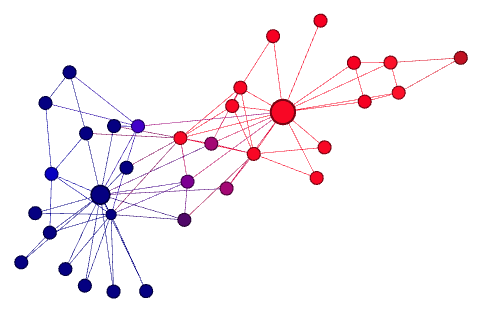
\includegraphics[width=0.4\textwidth]{karate.png}
    \caption{{Example of an image.}}
    \label{fig:karate}
\end{figure}


 




\bibliographystyle{IEEEtran}
\bibliography{bibliography}


\end{document}
